\subsection{Data Access Layer}
\paragraph*{Kommunikation med Central Server}
Klienten i Administrationssystemet består af en socketconnection som er defineret i SharedLib[Ref]. Da denne skal bruges i både businesslogic, men også i MainWindowViewModel og der samtidig øn-skes at den samme benyttes hver gang, bruges Singleton[Reference] for denne forbindelse. \\
Til at sende data benyttes en ModelHandler [Ref], som hver i sær har en metode til de forskellige handlinger. Eksempelvis EditProduct, DeleteProduct mf. Disse metoder arbejder alle sammen på samme måde:
\begin{enumerate}
\item Opret en XML-kommandostring vha. protokollen [\textbf{REFERENCE TIL PROTOKOLLEN}]
\item Send data til klienten
\end{enumerate}


\begin{figure}[!h]
    \centering
    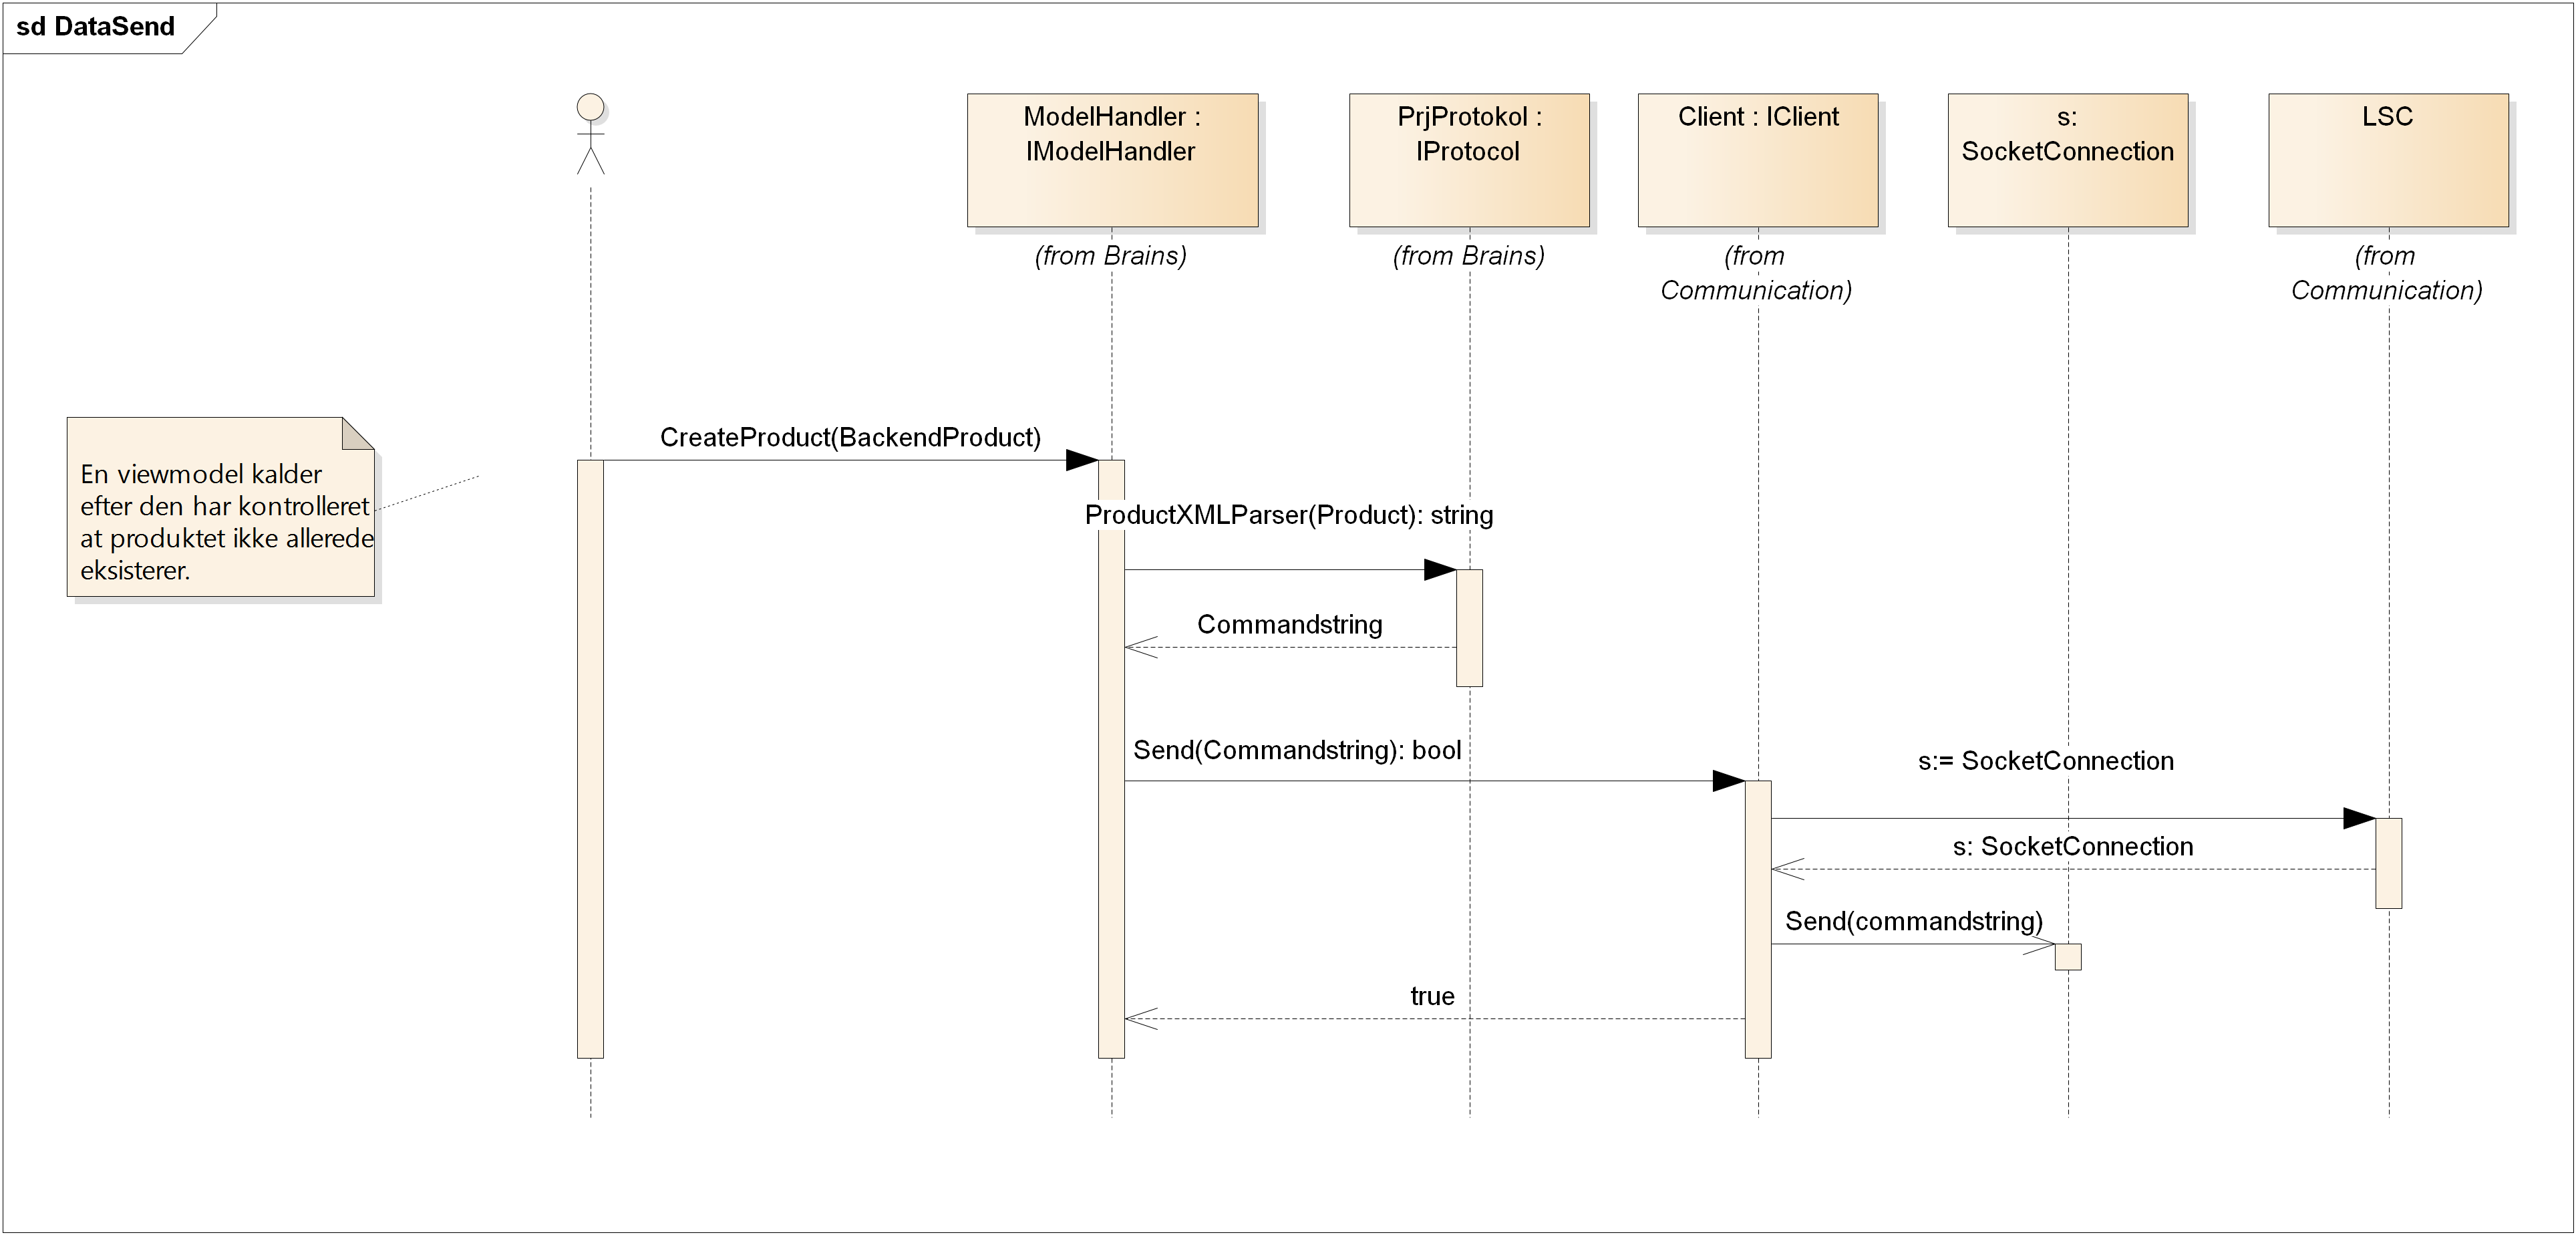
\includegraphics[width=1\textwidth]{Systemdesign/backend/Images/DataSend.png}
    \caption{Eksempel på hvordan CreateProduct bliver behandlet i systemet og sendt til Central Server}
    \label{fig:CreateSend}
\end{figure}

Derefter afsluttes der. Det betyder at når der eksempelvis oprettes et nyt produkt, bliver der ikke opdateret noget i systemet, der bliver udelukkende sendt data til serveren.\\\\


For at modtage data, subscriber MainWindowViewModel på nogle forskellige events, som eksempelvis OnProductCategoryDeleted, OnProductEdited mf. Dette gøres igennem klassen SocketEventHandlers [Ref], som også indeholder de eventhandlere der bliver kaldt, når et event raises på serveren.  Det er derfor disse eventhandlere som håndtere dataen, og lægger den nye data ind i datamodellerne – og det er først der, der bliver opdateret lokalt. På den måde vil der aldrig eksistere noget i databasen der ikke eksisterer i Administrationssystemet og vice versa. 
\begin{figure}[!h]
    \centering
    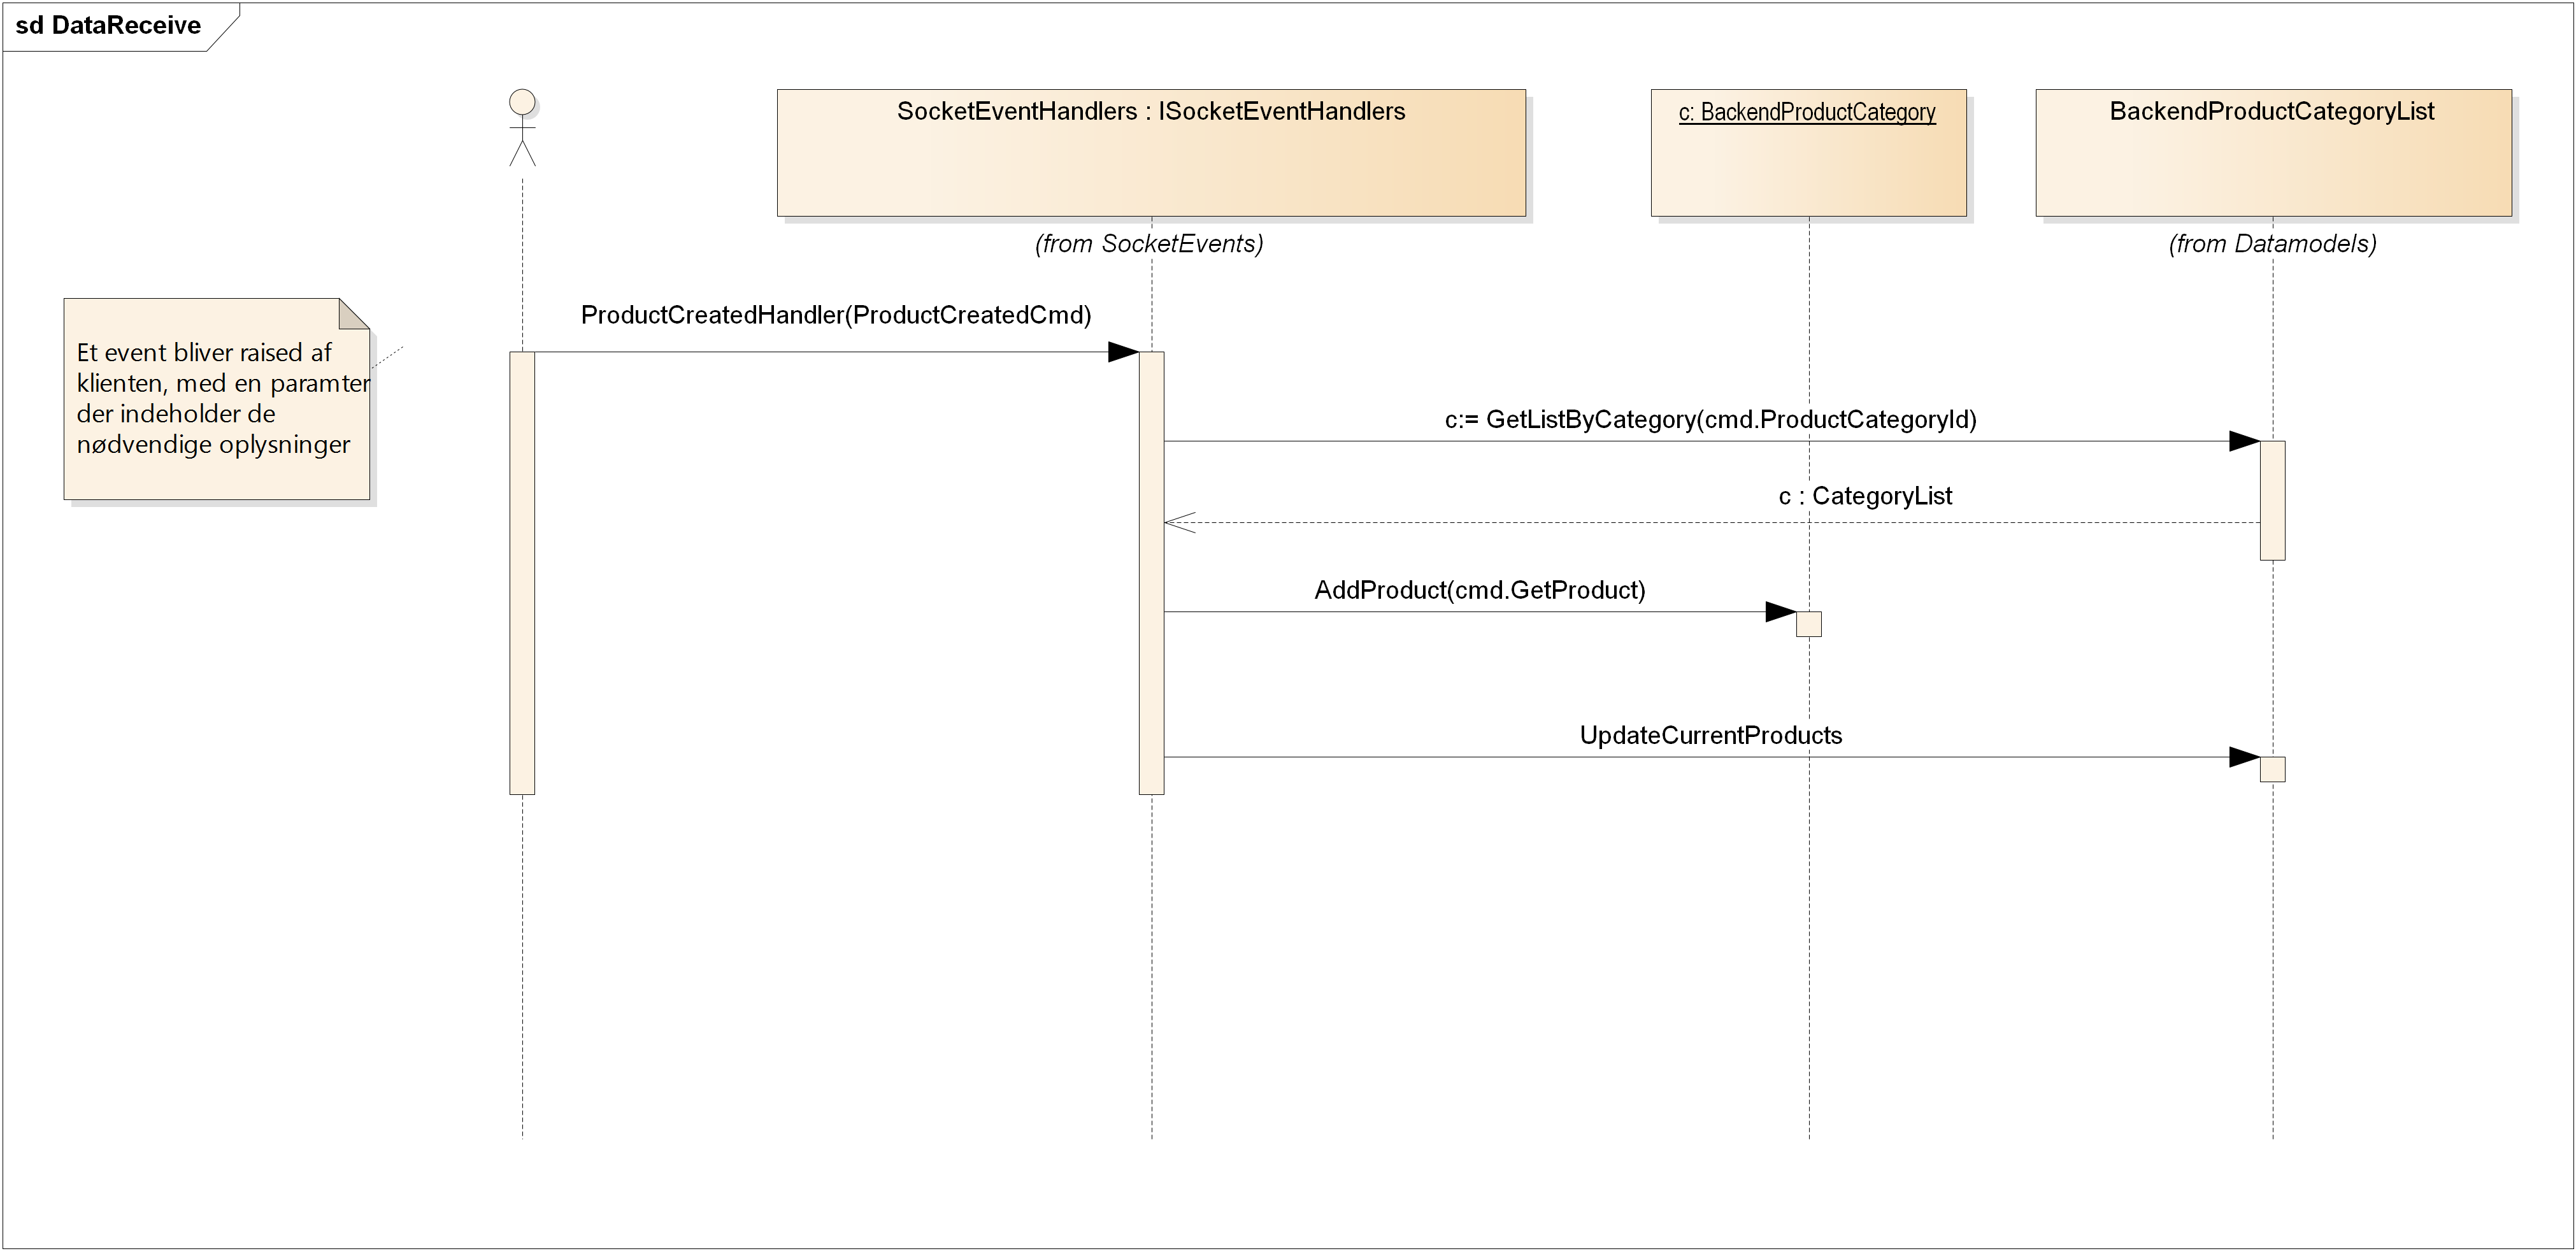
\includegraphics[width=1\textwidth]{Systemdesign/backend/Images/DataReceive.png}
    \caption{Eksempel på hvordan produktet igen bliver modtaget fra serveren, efter det er blevet oprettet.}
    \label{fig:DataReceive}
\end{figure}

